\documentclass[tikz,border=14pt]{standalone}
\usepackage[utf8]{inputenc}
\usepackage[T1]{fontenc}
\usepackage{lmodern}
\usepackage{amsmath}
\usetikzlibrary{arrows.meta,positioning,shapes.geometric,fit,backgrounds}

\definecolor{navy}{RGB}{24,58,92}
\definecolor{navyfill}{RGB}{236,243,250}
\definecolor{teal}{RGB}{15,118,110}
\definecolor{tealfill}{RGB}{234,248,246}
\definecolor{amber}{RGB}{180,83,9}
\definecolor{amberfill}{RGB}{254,245,231}
\definecolor{greenborder}{RGB}{27,94,32}
\definecolor{greenfill}{RGB}{235,247,237}
\definecolor{slate}{RGB}{71,85,105}
\definecolor{boxbg}{RGB}{248,250,252}

\begin{document}
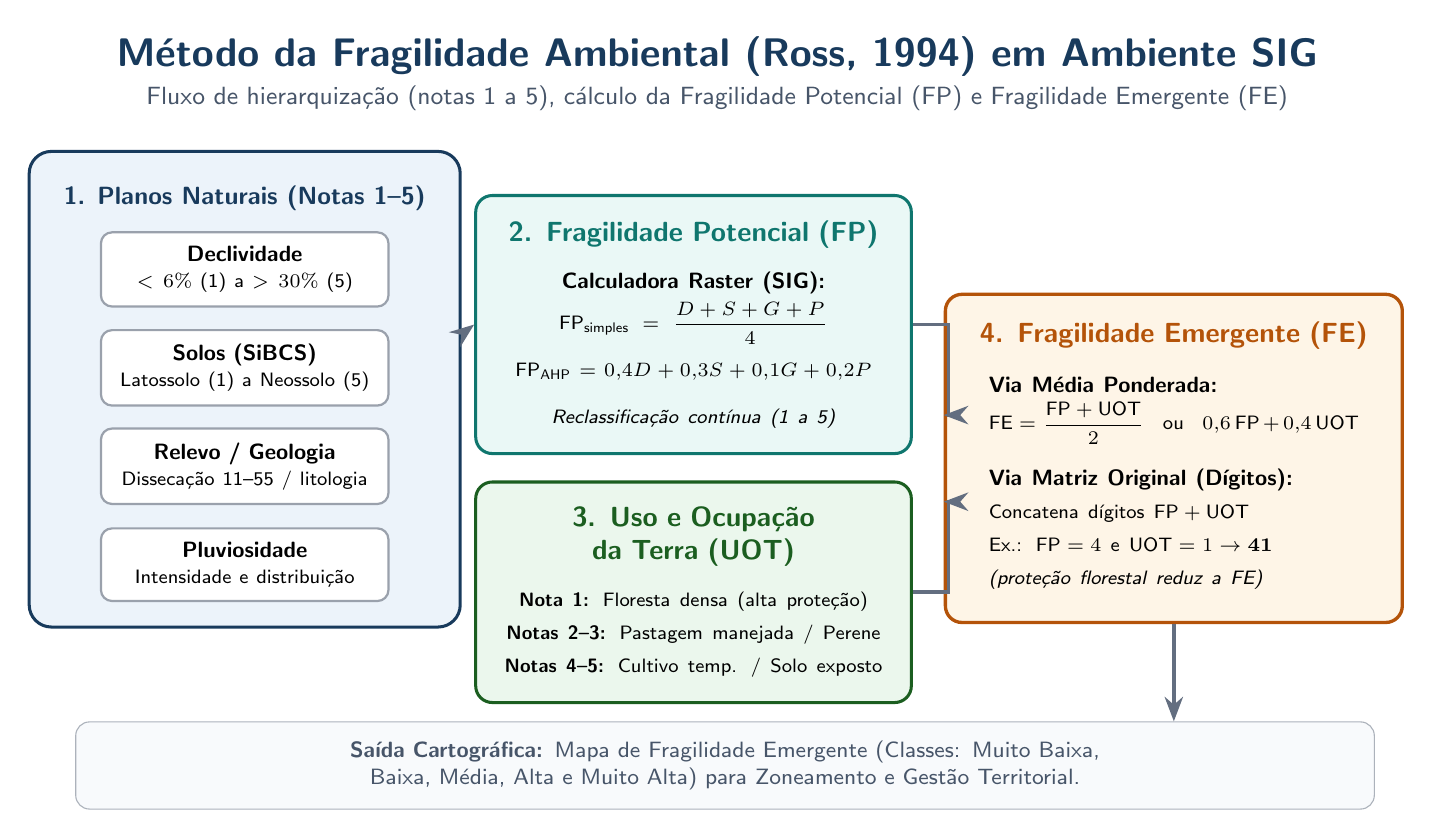
\begin{tikzpicture}[
  font=\sffamily,
  >=Stealth,
  title/.style={font=\sffamily\bfseries\Large, text=navy},
  subtitle/.style={font=\sffamily\small, text=slate},
  subbox/.style={
    rectangle, rounded corners=4pt, draw=slate!55, line width=0.8pt,
    fill=white, align=center, inner sep=5pt, font=\sffamily\footnotesize
  },
  arrow/.style={->, line width=1.3pt, color=slate!85}
]

% Cabeçalho
\node[title] (hdr) at (0, 5.45) {Método da Fragilidade Ambiental (Ross, 1994) em Ambiente SIG};
\node[subtitle] at (0, 4.92) {Fluxo de hierarquização (notas 1 a 5), cálculo da Fragilidade Potencial (FP) e Fragilidade Emergente (FE)};

% Etapa 1: Planos Naturais
\node[font=\sffamily\bfseries\small, text=navy] (lbl1) at (-6.0, 3.65) {1. Planos Naturais (Notas 1--5)};
\node[subbox, text width=3.3cm] (d) at (-6.0, 2.75) {\textbf{Declividade}\\{\scriptsize $<6\%$ (1) a $>30\%$ (5)}};
\node[subbox, text width=3.3cm] (s) at (-6.0, 1.50) {\textbf{Solos (SiBCS)}\\{\scriptsize Latossolo (1) a Neossolo (5)}};
\node[subbox, text width=3.3cm] (g) at (-6.0, 0.25) {\textbf{Relevo / Geologia}\\{\scriptsize Dissecação 11--55 / litologia}};
\node[subbox, text width=3.3cm] (p) at (-6.0, -1.00) {\textbf{Pluviosidade}\\{\scriptsize Intensidade e distribuição}};

\begin{scope}[on background layer]
  \node[rectangle, rounded corners=8pt, draw=navy, line width=1.1pt, fill=navyfill,
        fit=(lbl1)(d)(s)(g)(p), inner sep=9pt] (grp1) {};
\end{scope}

% Etapa 2: Fragilidade Potencial (FP)
\node[rectangle, rounded corners=6pt, draw=teal, line width=1.1pt, fill=tealfill,
      text width=4.9cm, align=center, inner sep=9pt] (fp) at (-0.3, 2.05) {
  \textbf{\color{teal}2. Fragilidade Potencial (FP)}\\[5pt]
  {\footnotesize \textbf{Calculadora Raster (SIG):}}\\[3pt]
  {\scriptsize $\text{FP}_{\text{simples}} = \dfrac{D + S + G + P}{4}$}\\[5pt]
  {\scriptsize $\text{FP}_{\text{AHP}} = 0{,}4D + 0{,}3S + 0{,}1G + 0{,}2P$}\\[5pt]
  {\scriptsize \textit{Reclassificação contínua (1 a 5)}}
};

% Etapa 3: Uso da Terra
\node[rectangle, rounded corners=6pt, draw=greenborder, line width=1.1pt, fill=greenfill,
      text width=4.9cm, align=center, inner sep=9pt] (uot) at (-0.3, -1.35) {
  \textbf{\color{greenborder}3. Uso e Ocupação da Terra (UOT)}\\[5pt]
  {\scriptsize \textbf{Nota 1:} Floresta densa (alta proteção)}\\
  {\scriptsize \textbf{Notas 2--3:} Pastagem manejada / Perene}\\
  {\scriptsize \textbf{Notas 4--5:} Cultivo temp. / Solo exposto}
};

% Etapa 4: Fragilidade Emergente (FE)
\node[rectangle, rounded corners=6pt, draw=amber, line width=1.2pt, fill=amberfill,
      text width=5.1cm, align=center, inner sep=10pt] (fe) at (5.8, 0.35) {
  \textbf{\color{amber}4. Fragilidade Emergente (FE)}\\[6pt]
  \begin{tabular}{@{}p{4.7cm}@{}}
    {\footnotesize \textbf{Via Média Ponderada:}}\\
    {\scriptsize $\text{FE} = \dfrac{\text{FP}+\text{UOT}}{2}$ \ ou \ $0{,}6\,\text{FP} + 0{,}4\,\text{UOT}$}\\[8pt]
    {\footnotesize \textbf{Via Matriz Original (Dígitos):}}\\
    {\scriptsize Concatena dígitos $\text{FP} + \text{UOT}$}\\
    {\scriptsize Ex.: $\text{FP}=4$ e $\text{UOT}=1 \rightarrow \mathbf{41}$}\\
    {\scriptsize \textit{(proteção florestal reduz a FE)}}
  \end{tabular}
};

% Rodapé síntese
\node[rectangle, rounded corners=5pt, draw=slate!45, fill=boxbg, text width=16.0cm,
      align=center, inner sep=7pt, font=\sffamily\footnotesize, text=slate] (rod) at (0.1, -3.55) {
  \textbf{Saída Cartográfica:} Mapa de Fragilidade Emergente (Classes: Muito Baixa, Baixa, Média, Alta e Muito Alta) para Zoneamento e Gestão Territorial.
};

% Setas limpas sem cruzamentos
\draw[arrow] ([yshift=0.7cm]grp1.east) -- (fp.west);
\draw[arrow] (fp.east) -- ++(0.45,0) |- ([yshift=0.55cm]fe.west);
\draw[arrow] (uot.east) -- ++(0.45,0) |- ([yshift=-0.55cm]fe.west);
\draw[arrow] (fe.south) -- (fe.south |- rod.north);

\end{tikzpicture}
\end{document}
